\subsection{\SOPT results with a broadened multiplicity range}\label{Sec:ResExpMult}

In Sec.~\ref{Sec:ResRat}, it was shown that the 0--1\% topology selection produced the largest effects, seen in Fig.~\ref{Fig:CombRatioPyEx} and Fig.~\ref{Fig:CombRatioHerEx}. However, the resonance particles had to be excluded in those measurements due to statistical limitations related to the signal extraction.
Therefore, in this Section, we report on \SOPT measurements with a broader multiplicity selection for the different \SOPT classes. We implement the broadening of the multiplicity estimation in two different ways:

\begin{enumerate}
    \item First, we broaden the midrapidity multiplicity estimation to 0--10\%, while simultaneously constricting the \SOPT event selection to the top 1\% quantile. This allows for a broader multiplicity range, while retaining the extreme topology selection, gaining a factor 10 in the number of events.
    
    \item Secondly, we investigate top-1\% multiplicity at forward rapidity in 0--10\% \SOPT quantiles. This is  to study the impact of a broader $\langle \rm{d}\it{N}_{\pi}/\rm{d}\it{y} \rangle$, and to compare midrapidity to forward rapidity multiplicity estimation between roughly similar \dndeta, as is seen in Fig.~\ref{Fig:CL1vsV0M}.
\end{enumerate}

Fig.~\ref{Fig:DRCL1} illustrates the \SOPT-differential ratios to $(\pi^+ + \pi^-)$ with multiplicity measured at midrapidity, with a simultaneous broadened multiplicity (\tracklet 0--10\%) and tightened \SOPT selection criteria, compared to the measurement presented in Sec.~\ref{Sec:ResRat}. The experimental data is compared with both PYTHIA 8.2 Ropes and EPOS-LHC,  which, as shown in previous sections of this article, give the most accurate predictions of the observed trends.

The double ratios for \KSTAR suggest that the production in isotropic topologies is similar to that of average high-multiplicity events. In contrast, there is a pronounced structure of the ratio for jet-like topologies, highlighting an overall suppression of \KSTAR production. The \PHI has similar features: suppression in jet-like events (qualitatively the same trend as for \XI), and consistent with unity for isotropic events. For all presented particle species, an overall narrower \SOPT selection highlights a large suppression of the \pt-differential yield of strange hadrons relative to pions in events with extreme jet-like topologies. Furthermore, there is a larger deviation among the four different models compared to the more constrained multiplicity quantile, in particular in jet-like topologies for protons, \XI, and \KSTAR. However, the overall trends are well predicted. Both resonance particles favor production in softer events containing QGP-like features, where the decrease of \KSTAR production in jet-like events could potentially be due to a rescattering effect. While the origin of the suppression of $\phi$ production in jet-like events is not fully understood, the behavior is consistent with the strange particles measured in this study.

The particle ratios to $(\pi^+ + \pi^-)$ for events with forward rapidity multiplicity estimations are presented in 0--10\% \SOPT event classes in Fig.~\ref{Fig:DRV0M}. The reported effects of \SOPT event-selection while estimating multiplicity through the V0M is comparatively weak to either percentile of tracklets, both for the looser and stricter \SOPT criteria. The PYTHIA 8.2 rope hadronization framework is able to accurately describe the interplay between different \SOPT event classes, while estimating multiplicity in the 
%
%
\begin{figure}[htbp!]
    \centering
        \hspace*{-1cm}
	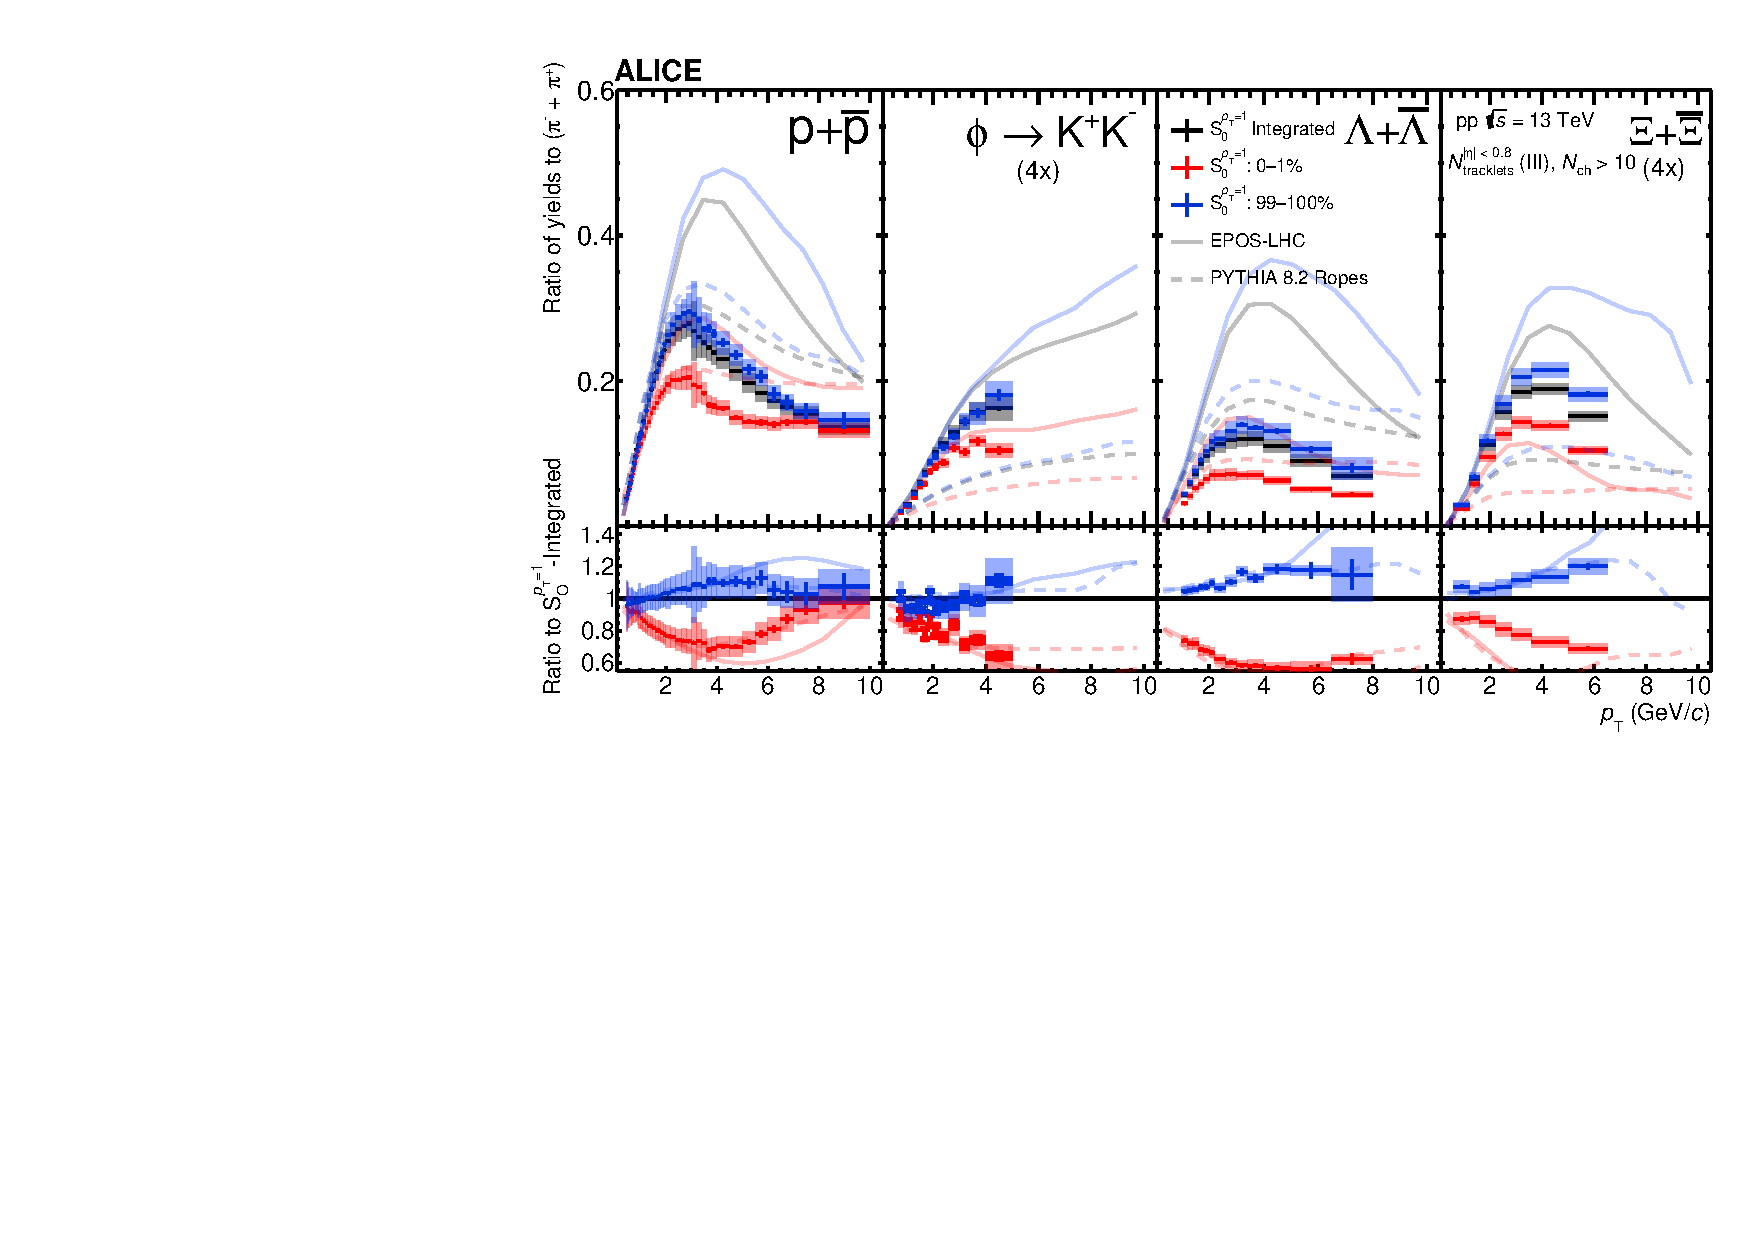
\includegraphics[scale=0.87]{figures/Baryons_SOPT_1_NSPD_10_EP.pdf}
	\newline
	\hspace*{-1cm}
	    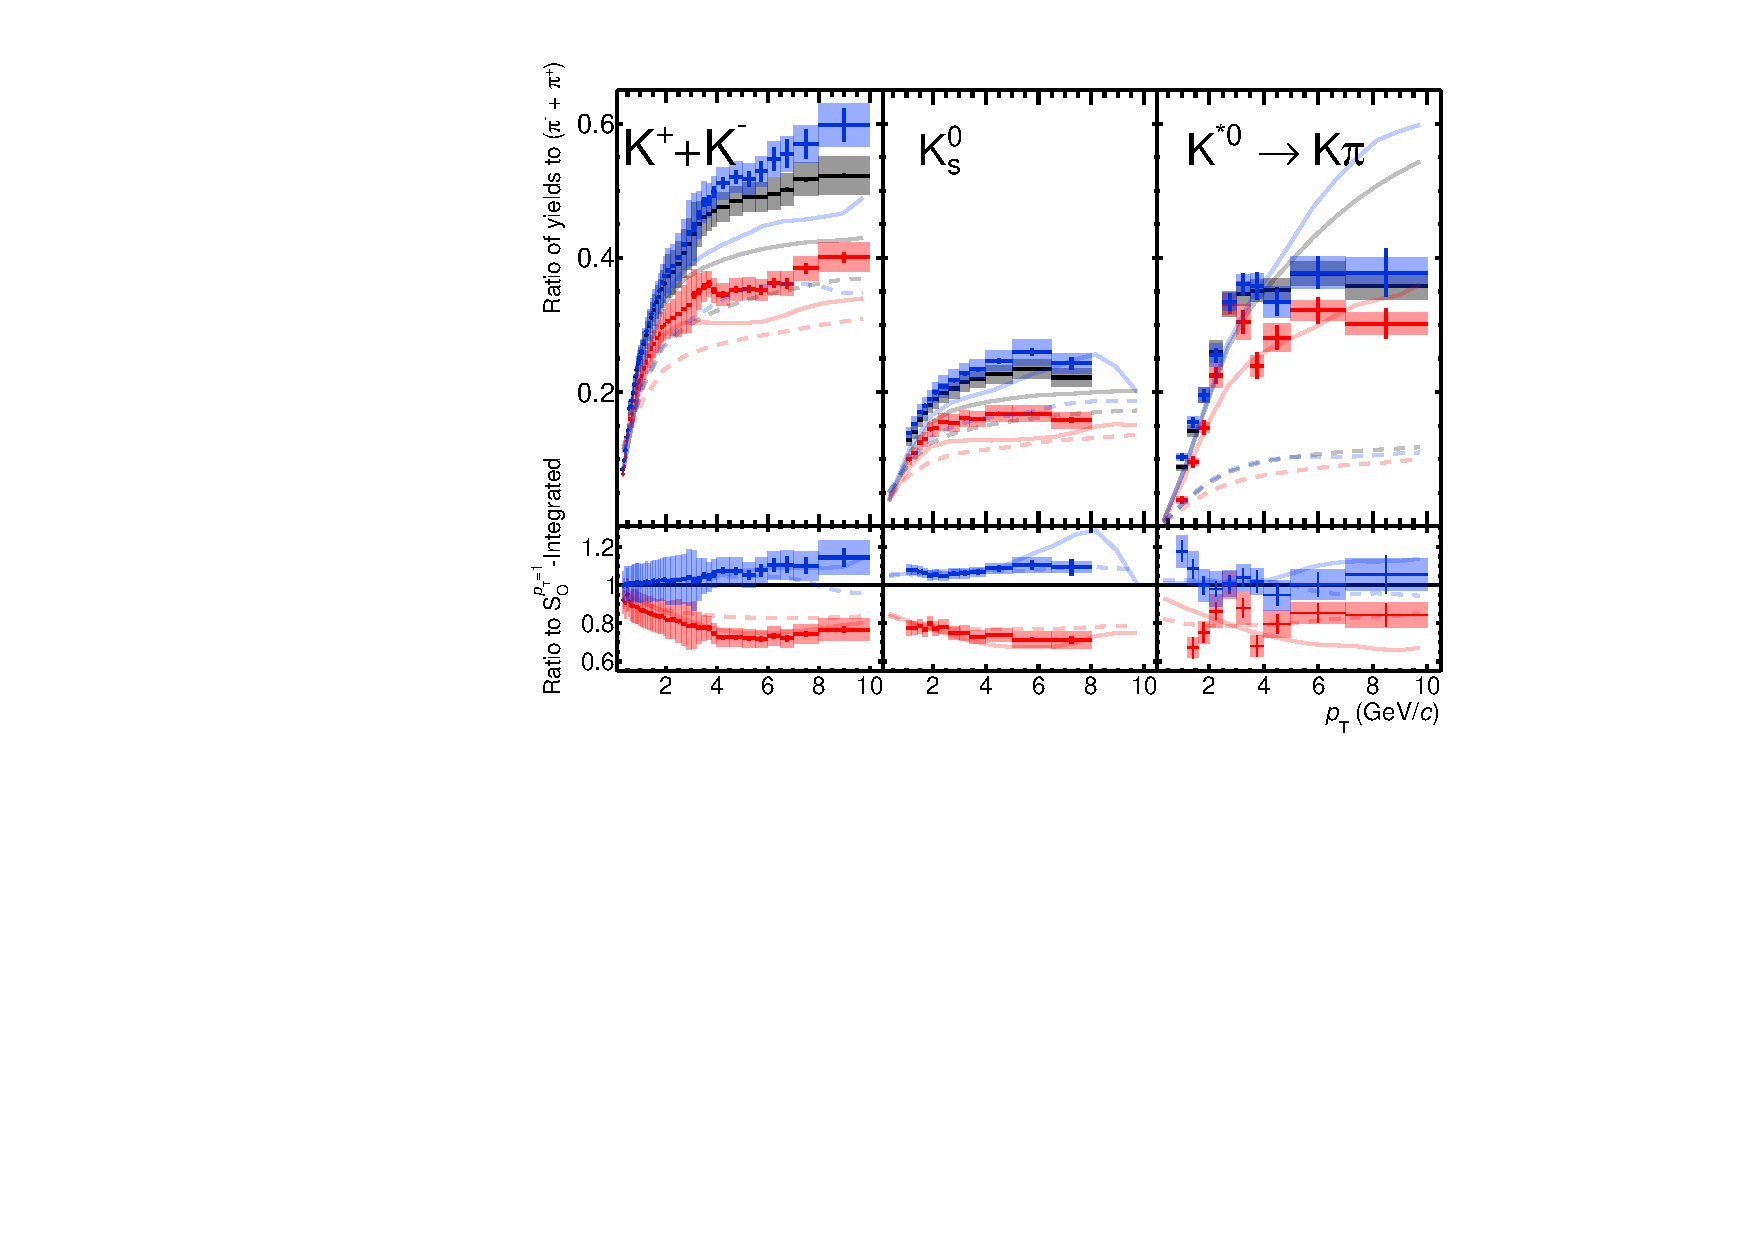
\includegraphics[scale=0.87]{figures/Mesons_SOPT_1_NSPD_10_EP.pdf}
  \caption{Top panels show hadron-to-\PI ratios for 0--1\% \SOPT classes selected for the 0--10\% \tracklet multiplicity events. Bottom panels present the hadron-to-\PI double-ratios of \SOPT classes relative to \SOPT integrated high-multiplicity events. Statistical and systematic uncertainties are shown by  bars and boxes, respectively. Experimental results are compared with predictions from EPOS-LHC and PYTHIA 8.2 Rope hadronization framework.}
   \label{Fig:DRCL1}
\end{figure}
%
%
\begin{figure}[htbp!]
    \centering
	\hspace*{-1cm}
	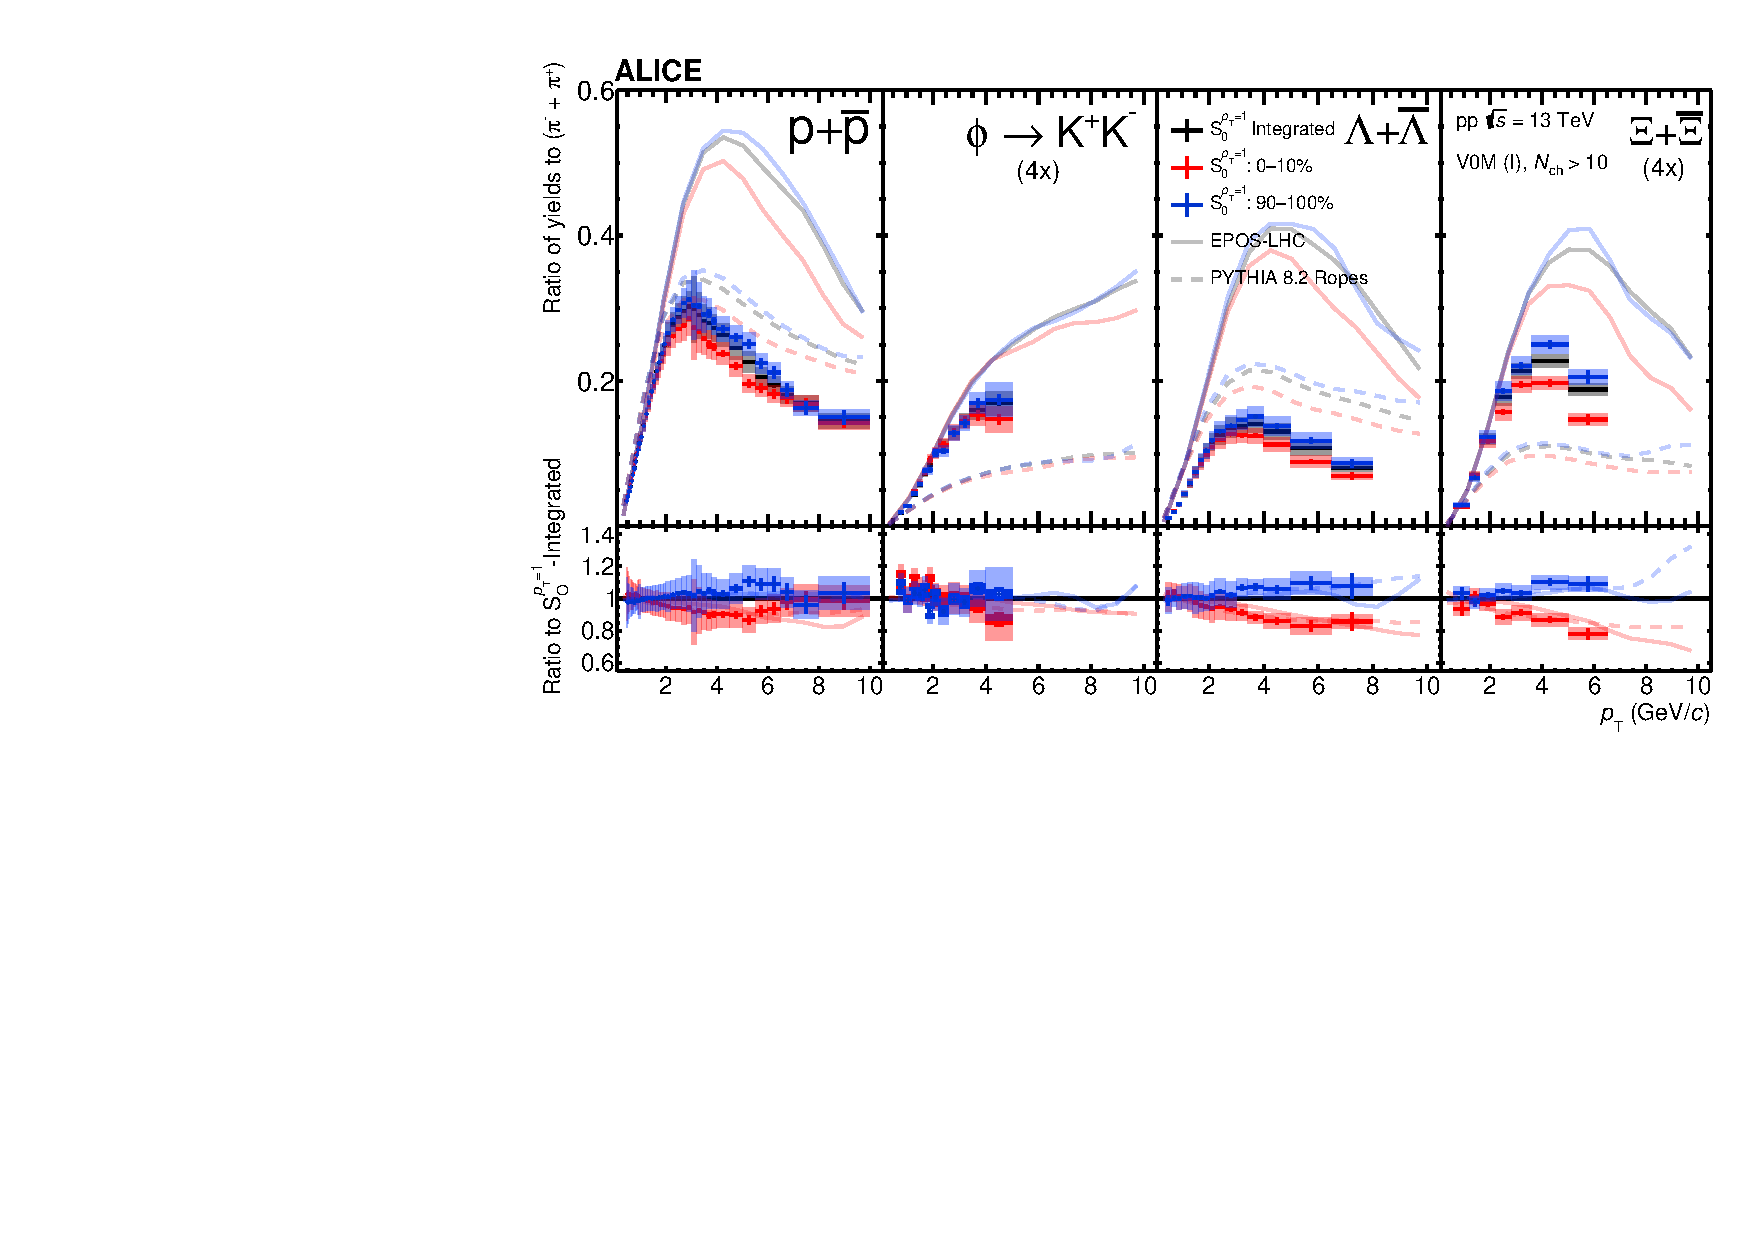
\includegraphics[scale=0.87]{figures/Baryons_SOPT_10_V0M_1_EP.pdf}
	\newline
	\hspace*{-1cm}
	 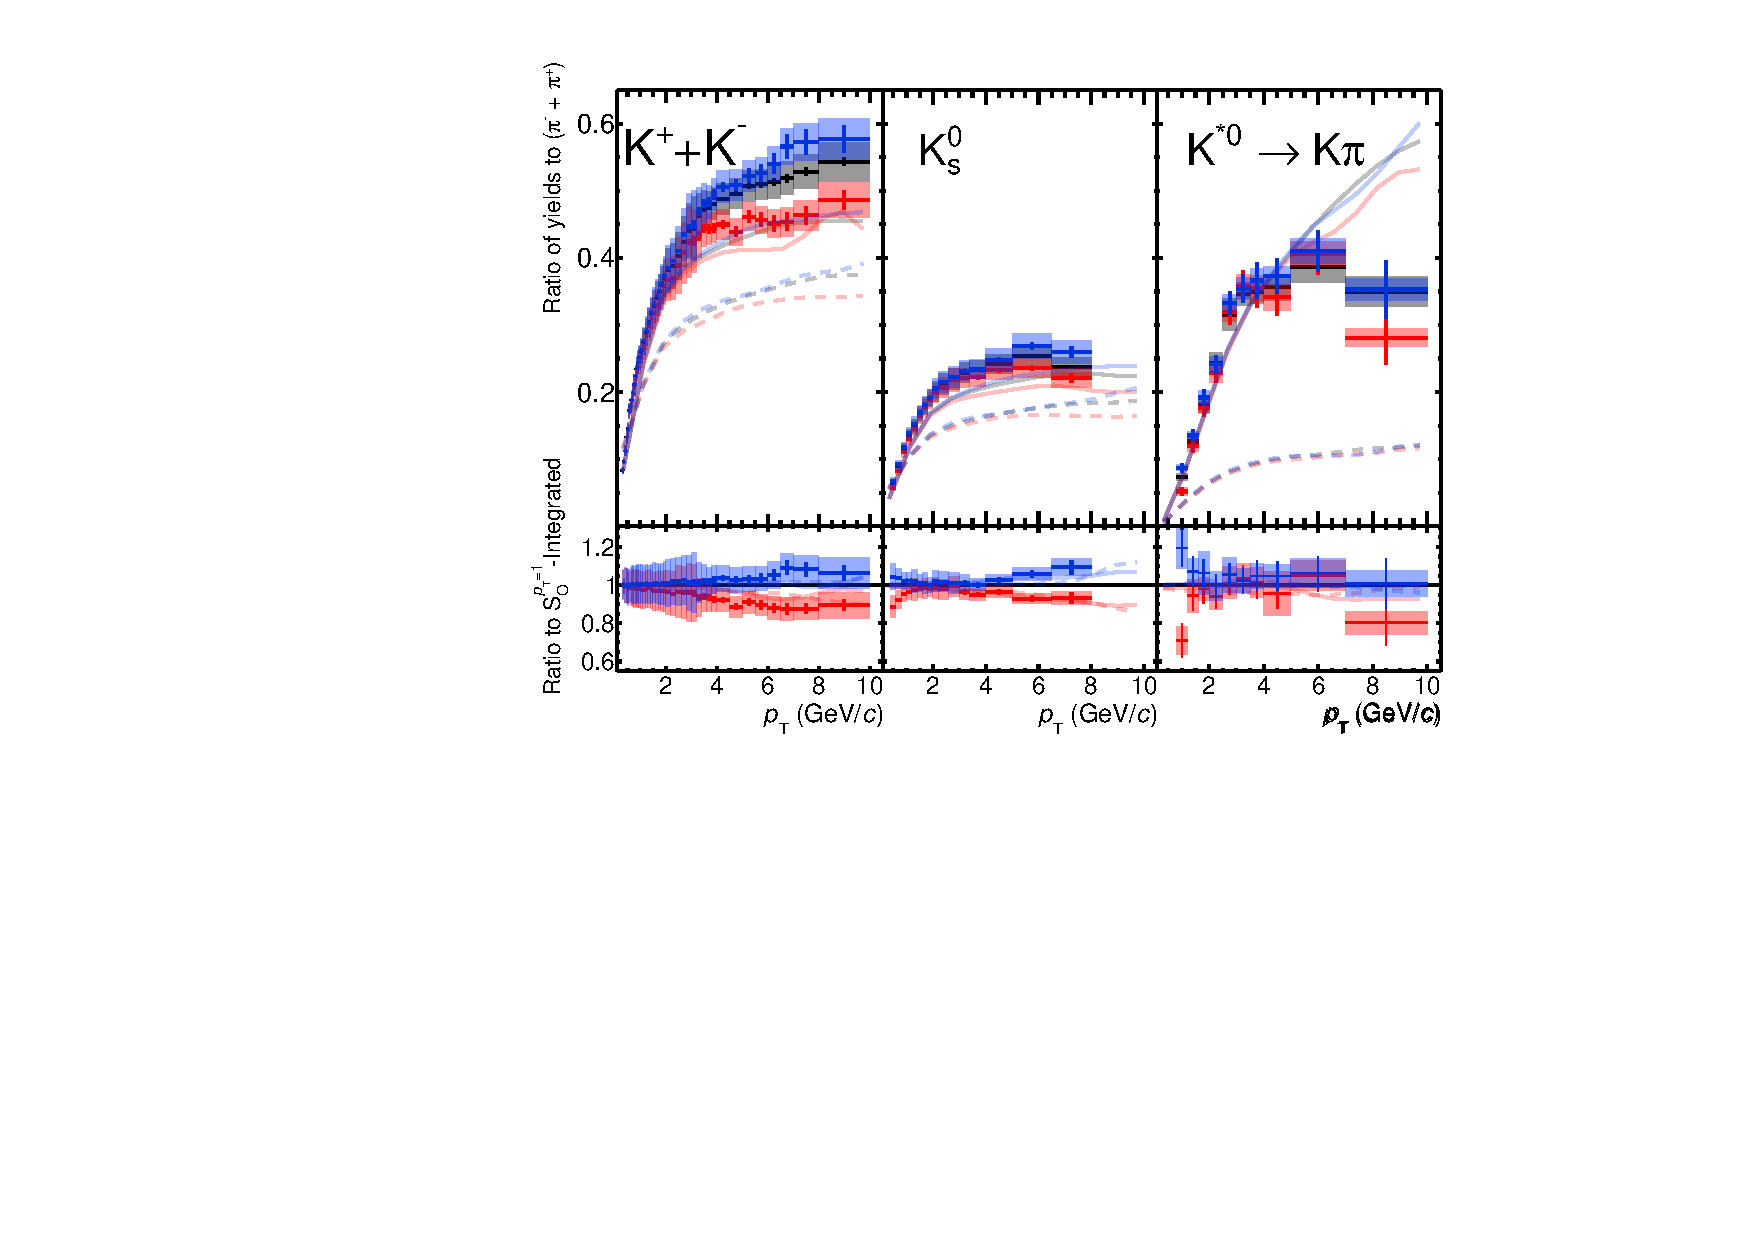
\includegraphics[scale=0.87]{figures/Mesons_SOPT_10_V0M_1_EP.pdf}
  \caption{Top panels show hadron-to-\PI ratios for 0--10\% \SOPT classes selected for the 0--1\% V0M multiplicity events. Bottom panels present the hadron-to-\PI double-ratios of \SOPT classes relative to \SOPT integrated high-multiplicity events. Statistical and systematic uncertainties are shown by  bars and boxes, respectively. Experimental results are compared with predictions from EPOS-LHC and PYTHIA 8.2 Rope hadronization framework.}
   \label{Fig:DRV0M}
\end{figure}
 forward rapidity region. In contrast, EPOS-LHC overestimates the relative enhancement and suppression of \XI and \LA in isotropic and jet-like topologies, respectively. The midrapidity multiplicity estimations (both 0--1\% and 0--10\%) showcase an increased sensitivity of strange hadron production as a function of \SOPT compared to the forward rapidity multiplicity estimation, even though the fractional $\langle \rm{d}\it{N}_{\pi}/\rm{d}\it{y} \rangle$ difference between the \SOPT event classes in this case are similar. This finding suggests that the effects of the relative enhancement (suppression) of light-flavor hadron production to \PI mesons in isotropic (jet-like) topologies are smaller while estimating multiplicity with V0M, and that one can study different physical properties relative to the rapidity ranges in which the multiplicity is estimated. 

Finally, in Fig.~\ref{Fig:V0M_1_Int} the \pt-integrated yields are presented as a function of \SOPT following the two expanded multiplicity estimations. It was shown in Sec.~\ref{Sec:IntYield} that the results utilizing the measured \pt ranges were consistent with yields obtained from integrating over the full, extrapolated \pt range. Therefore, for the sake of brevity, this section will only include yields integrated over the measured \pt ranges, to allow for maximal precision when compared with model predictions.  Remarkably, the \SOPT-dependent enhancement of strange hadrons seems to vanish once the multiplicity estimation is performed at forward rapidity. Similarly to Figs.~\ref{Fig:CL1_1_Int_py} and ~\ref{Fig:CL1_1_Int_hw}, the effect of strangeness enhancement is consistent between different ranges of the midrapidity multiplicity estimation, and the effect is suggested to be slightly stronger in the more extreme multiplicity case.


\begin{figure}[ht!]
    \vspace{0.1cm}
    \centering
    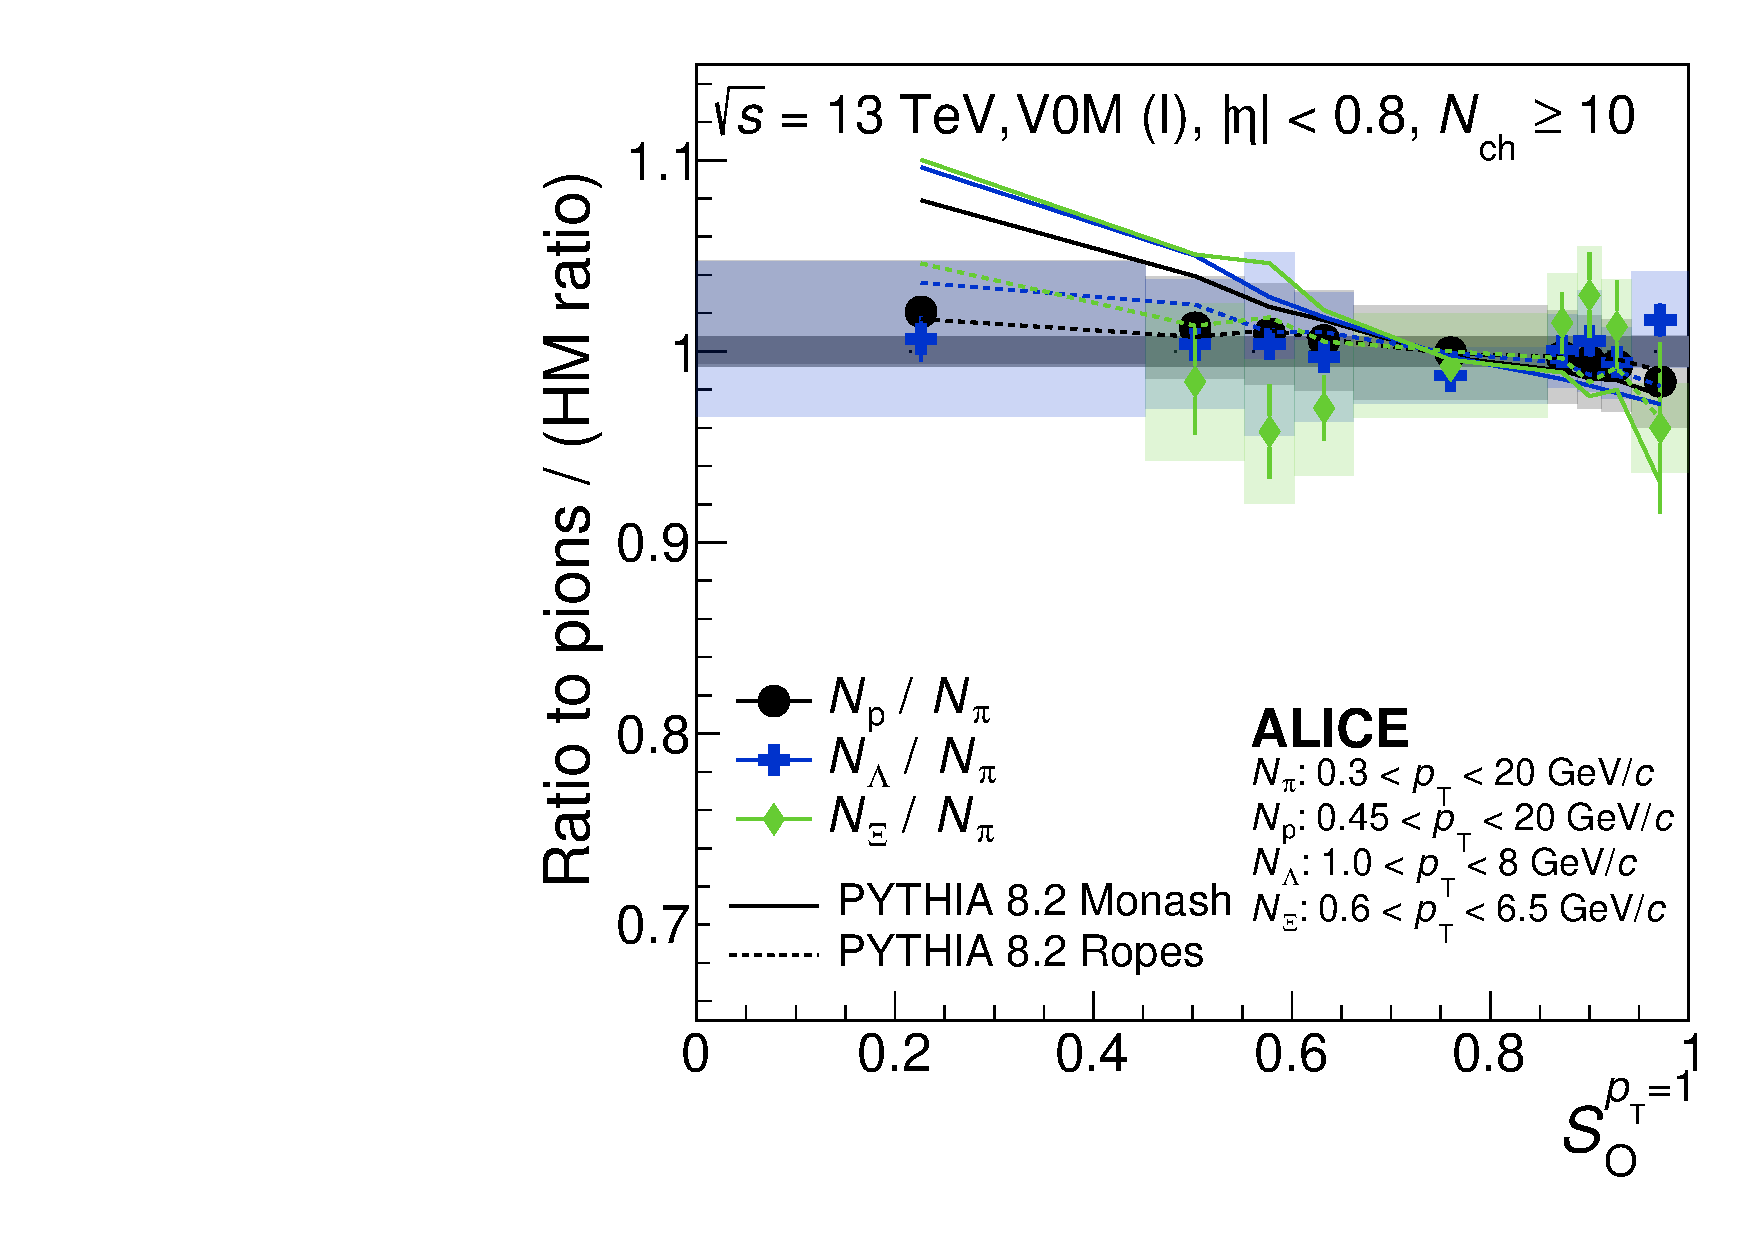
\includegraphics[scale=0.36]{figures/xi_over_pi_vs_So_V0M_01_PY.pdf}
    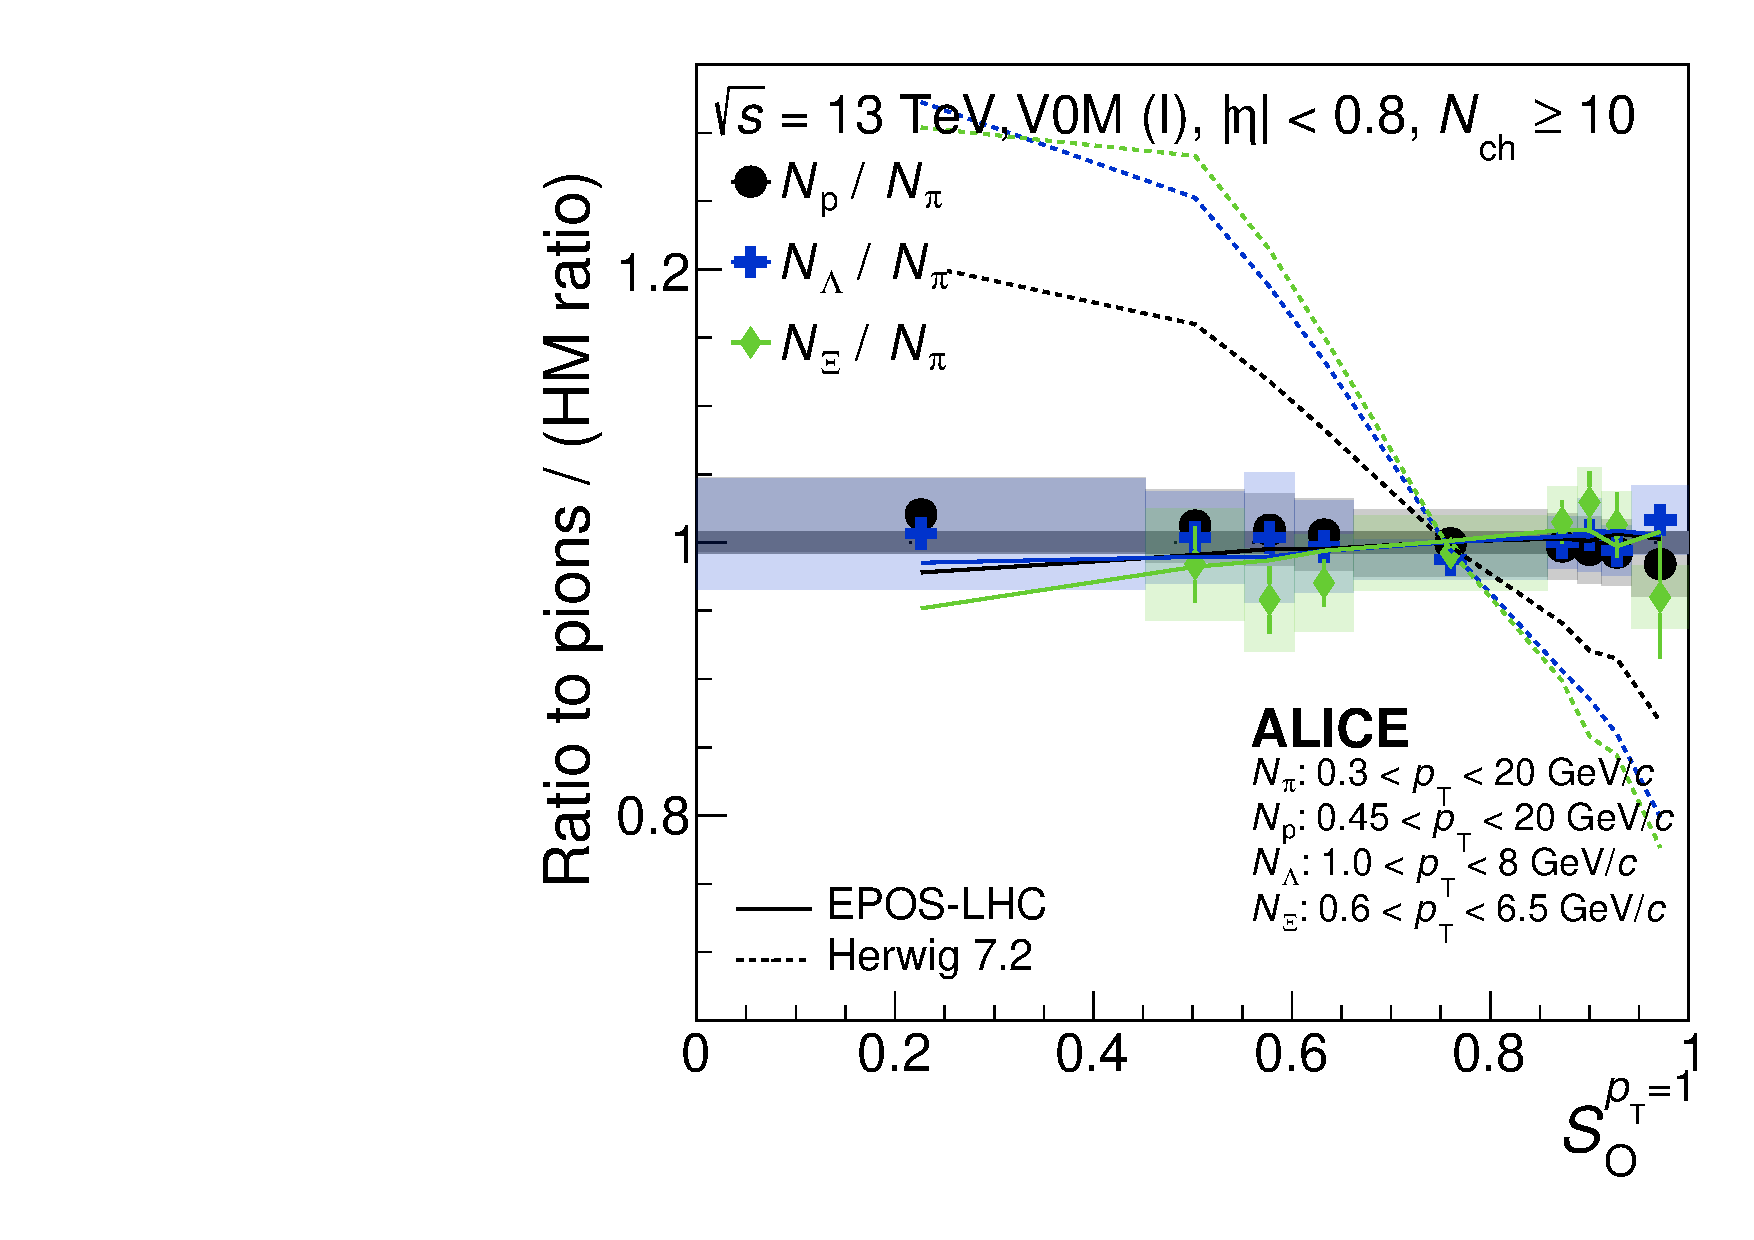
\includegraphics[scale=0.36]{figures/xi_over_pi_vs_So_V0M_01_HW.pdf}
    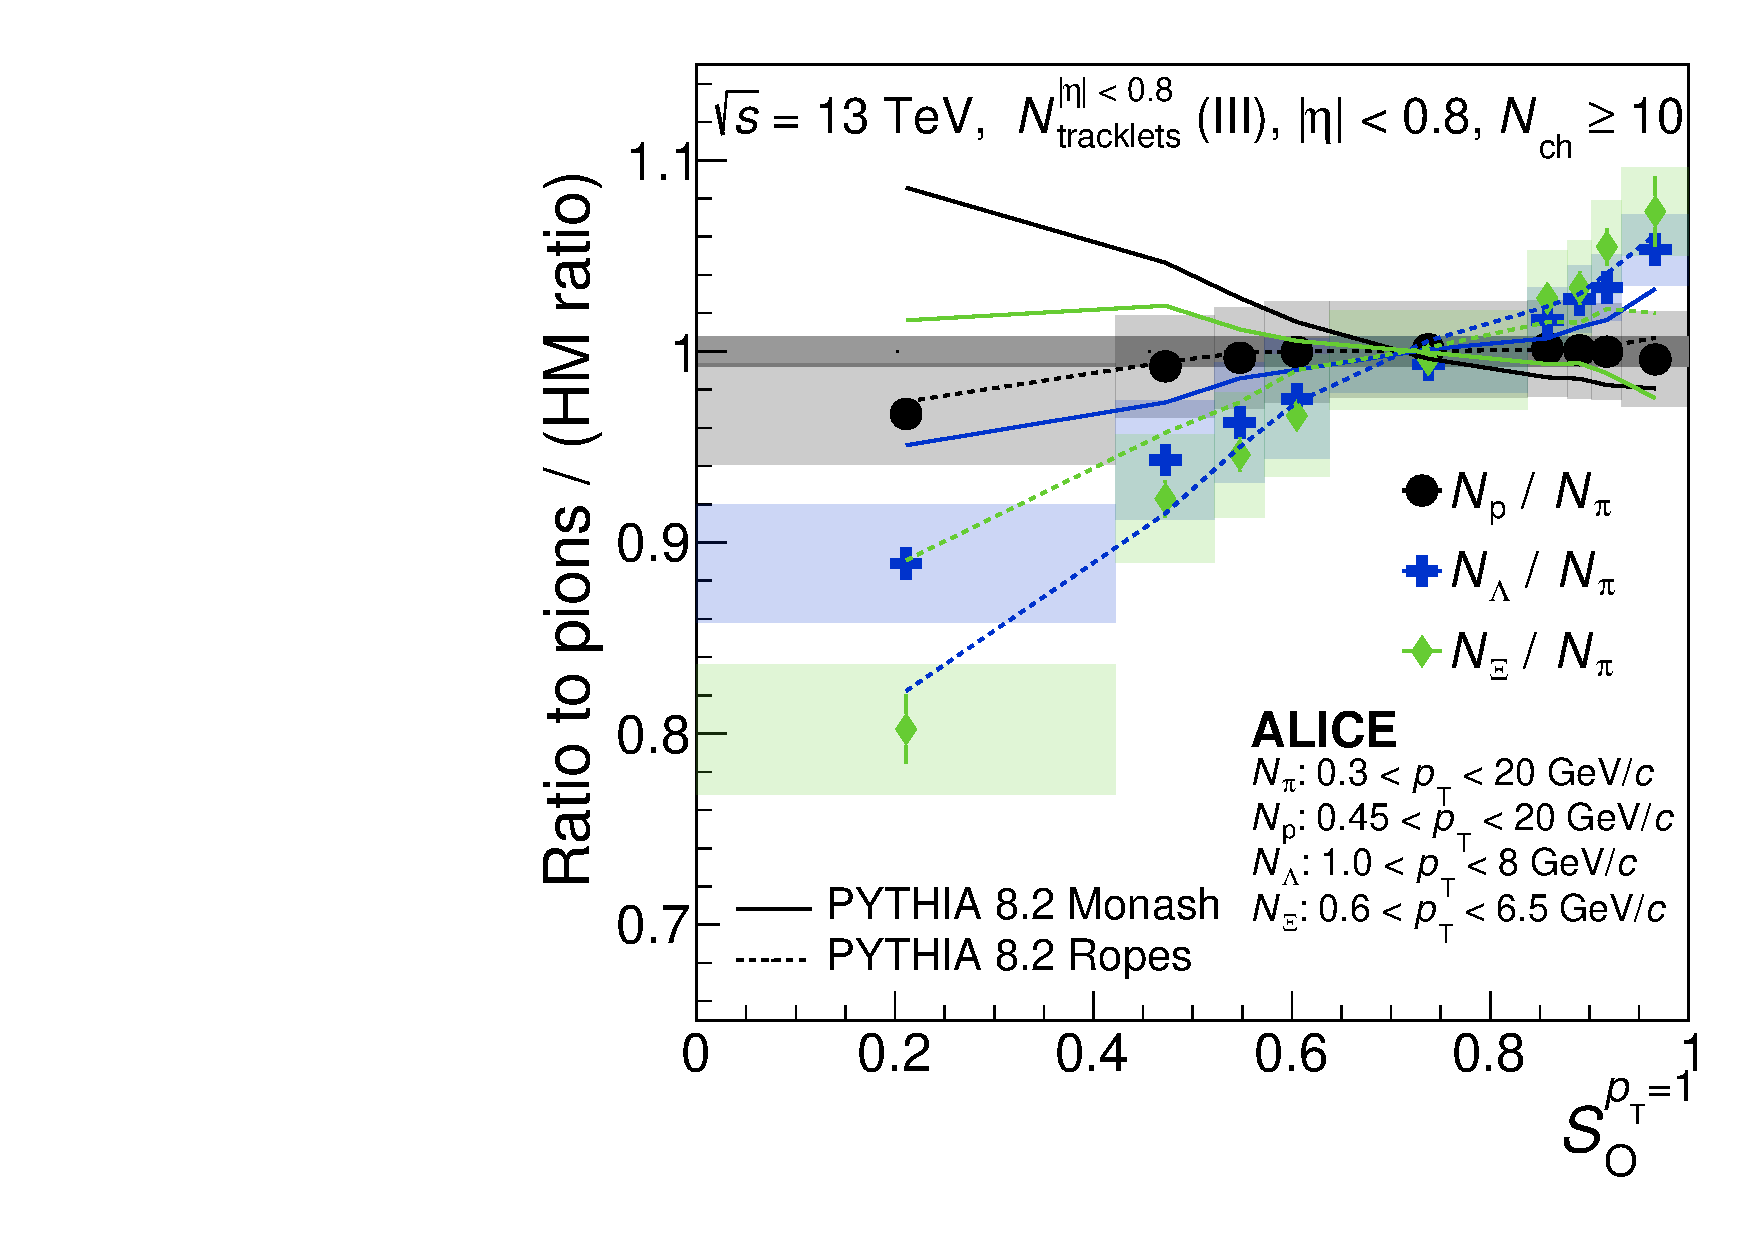
\includegraphics[scale=0.36]{figures/xi_over_pi_vs_So_CL1_10_PY.pdf}
    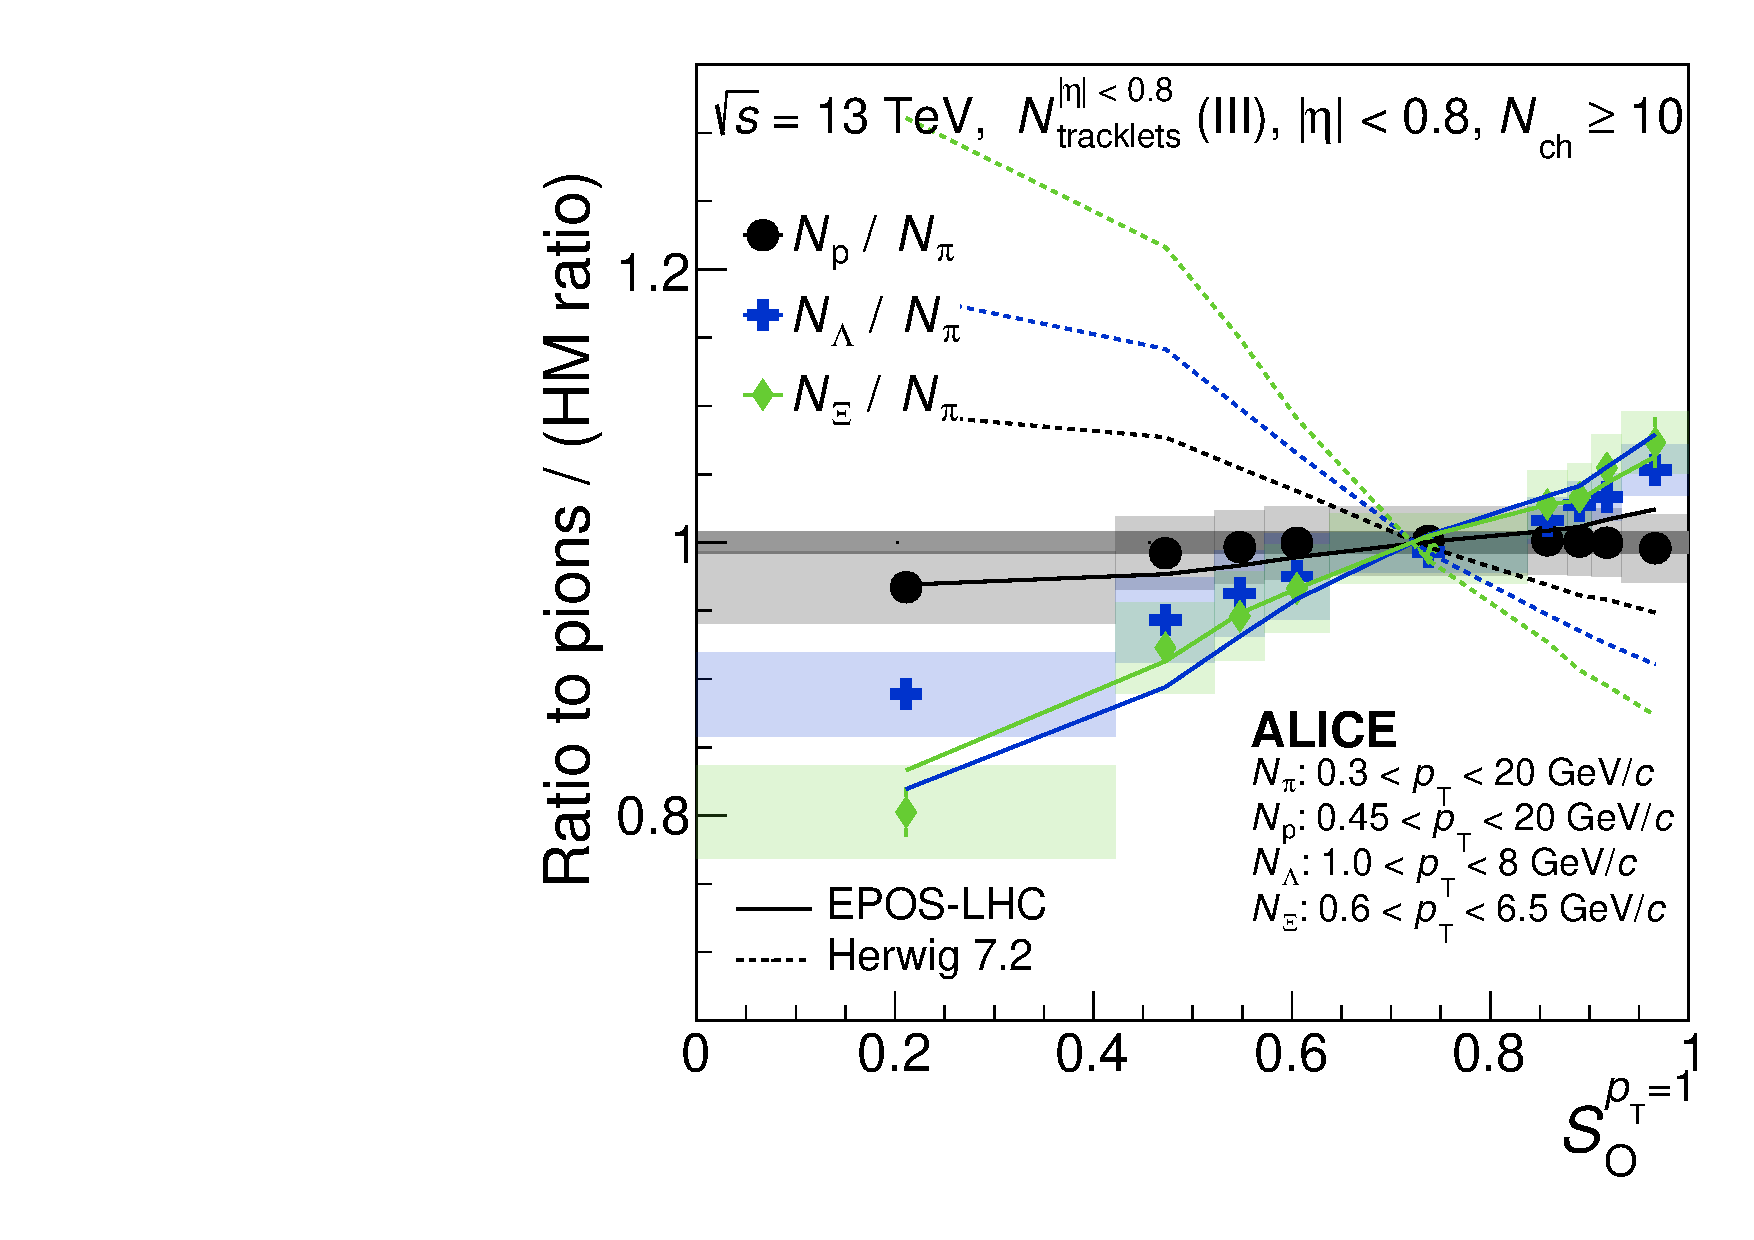
\includegraphics[scale=0.36]{figures/xi_over_pi_vs_So_CL1_10_HW.pdf}
    \caption{The double ratios of integrated yield as a function of \SOPT are presented for V0M 0--1\% (upper) and \tracklet 0--10\%  (lower). Left and right panels show the same data points, but with different model predictions. Statistical and total systematic uncertainties are shown by bars and boxes, respectively. The curves represent different model predictions of the same measurement. }
    \label{Fig:V0M_1_Int}
\end{figure}


Both EPOS-LHC and the PYTHIA 8.2 rope hadronization framework are able to qualitatively describe the enhancement of \LA and \XI with increasing \SOPT, while simultaneously predicting the insensitivity of strange particle production as a function of \SOPT when estimating multiplicity at forward rapidity. 


Finally, due to the increase of the number of events from the broader multiplicity interval, it is possible to measure the integrated $\phi$ over the full \SOPT range. This is presented in Fig.~\ref{Fig:CL1_10_Int_phi}, where integrated \PHI yields are compared to \XI yields as function of \SOPT, for \tracklet 0--10\%, relative to the equivalent ($\pi^+\pi^-$) yields. It is observed that there is no significant modification of the relative \PHI meson yield as a function of \SOPT within systematic uncertainties. This is in clear contrast to the features exhibited when measuring the relative \XI production. Given the similarity of the proton curves in Fig.~\ref{Fig:V0M_1_Int}, these results imply that the $\phi$ meson has the properties of particles with net-zero strangeness content when measured as a function of \SOPT. The resulting suppression or enhancement of relative hadron yields as a function of \SOPT are therefore suggested to be driven by the hadron mass, rather than by the effective strangeness of the hadron.

The data is compared to PYTHIA 8.2 ropes and EPOS-LHC, both able to quantitatively predict the dynamics of the relative $\phi$ yields as a function of \SOPT. However, in PYTHIA 8.2, one would naively expect that the \PHI dynamics should follow the same trend as \XI, as both are effectively double-strange. This observed difference suggests that the \XI enhancement in the PYTHIA 8.2 rope model can mainly be attributed to addition of Junction formations, which only enhances baryon production.

\begin{figure}[t]
    \vspace{0.1cm}
    \centering
    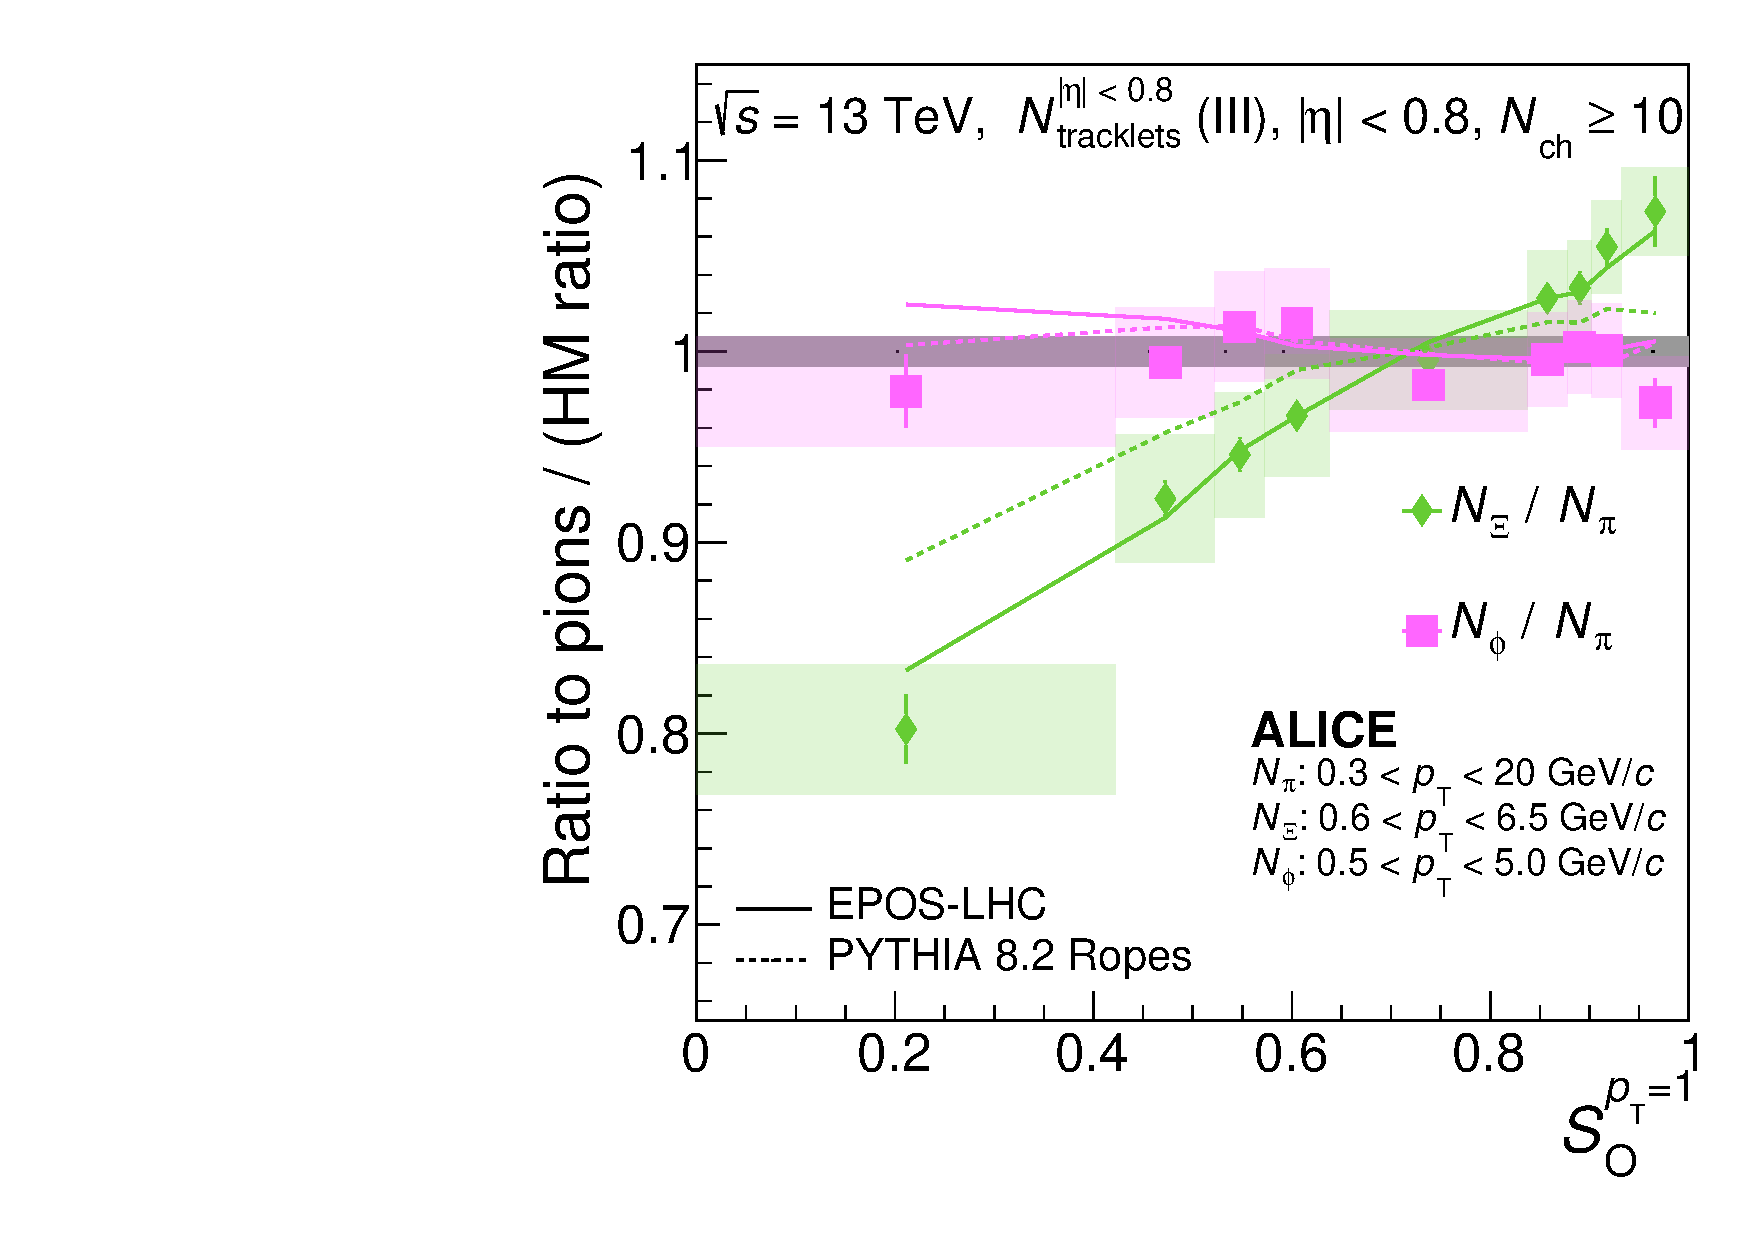
\includegraphics[scale=0.75]{figures/xi_over_pi_vs_So_CL1_10_EP.pdf}
    \caption{The double ratios of integrated yield as a function of \SOPT in \tracklet 0--10\% for $\phi$ and \XI. Statistical and total systematic uncertainties are shown by bars and boxes, respectively. The curves represent different model predictions of the same measurement}
    \label{Fig:CL1_10_Int_phi}
\end{figure}
